\documentclass[a4paper,10pt]{scrartcl}
%encodings
\usepackage[utf8]{inputenc}
\usepackage[english]{babel}
\usepackage[T1]{fontenc}
%colors, hyperrefs
\usepackage{color}
\usepackage{url}
\usepackage[pdftex,pdfauthor={J\"org Behrmann, Anika Haller},pdftitle={Ma10: Auger- and Electron Energy Loss Spectroscopy}]{hyperref}
%figures and subfigures
\usepackage[pdftex]{graphicx}
\usepackage{subfigure}
%better tables
\usepackage{tabularx}
\usepackage{booktabs}
\usepackage{multirow}
%math stuff
\usepackage{amsmath}
\usepackage{amsthm}
\usepackage{amsfonts}
\usepackage{IEEEtrantools}
\usepackage[square,comma,numbers,sort&compress]{natbib}
%shiny stuff
\usepackage[babel]{microtype}
\DisableLigatures{encoding=T1,family=tt*}

\usepackage{verbatim}

\begin{document}

\title{Ma10: Auger- and Electron Energy Loss Spectroscopy}
\author{J\"org Behrmann\footnote{behrmann@physik.fu-berlin.de} \qquad Anika Haller\footnote{halleran@zedat.fu-berlin.de}}
\date{31.10.2011}
\maketitle
\tableofcontents
\thispagestyle{empty}

\clearpage

\section{Introduction}

In 1922 Lise Meitner first described the effect that from 1923 on would carry Pierre Augers name. For many years the features of the Auger effect were a nuisance to X-ray spectroscopists, thought to not carry any useful information. This view has since changed in the last half-centennial and Auger spectroscopy has thus become a very useful source of information about surface effects, due to the very short mean free path of low-energy electrons in most materials. Thus these electrons cannot penetrate the material very deeply, which makes this spectroscopic technique very surface sensitive. Furthermore, the resulting spectra are specific to the materials analyzed, therefore we will use the Auger effect in the present experiment to measure impurities on the surface of a sample and to later ascertain the material of our sample.

Even for energies that cannot lead to Auger excitation electrons do scatter inelastically. The energy and deflection angle of deflected electrons can then be used to gain information about the scatterer, e.g. phonons or plasmons, with which the electron has scattered. This closely related spectroscopic technique is called Electron Energy Loss Spectroscopy (EELS) and will be used in the our experiment to analyze surface plasmons.

\subsection{Universal Curve of Escape Depth}

Figure~\ref{fig:ucurve} shows the universal curve of electron escape depth, which shows that that the depth from which an incoming electron can escape from a surface again is only dependent on the electron's energy and thus more or less independent of the material. This universal curve can be obtained on theoretical grounds by considering that first for increasing energy (up to $70\,$eV) more and more interaction modes, e.g. phonon modes, become available as potential scatterers to the incoming electron, which decreases the particles mean free path. Whereas for even higher energies the excess energy can be used to penetrate the material further.

\begin{figure}
\centering
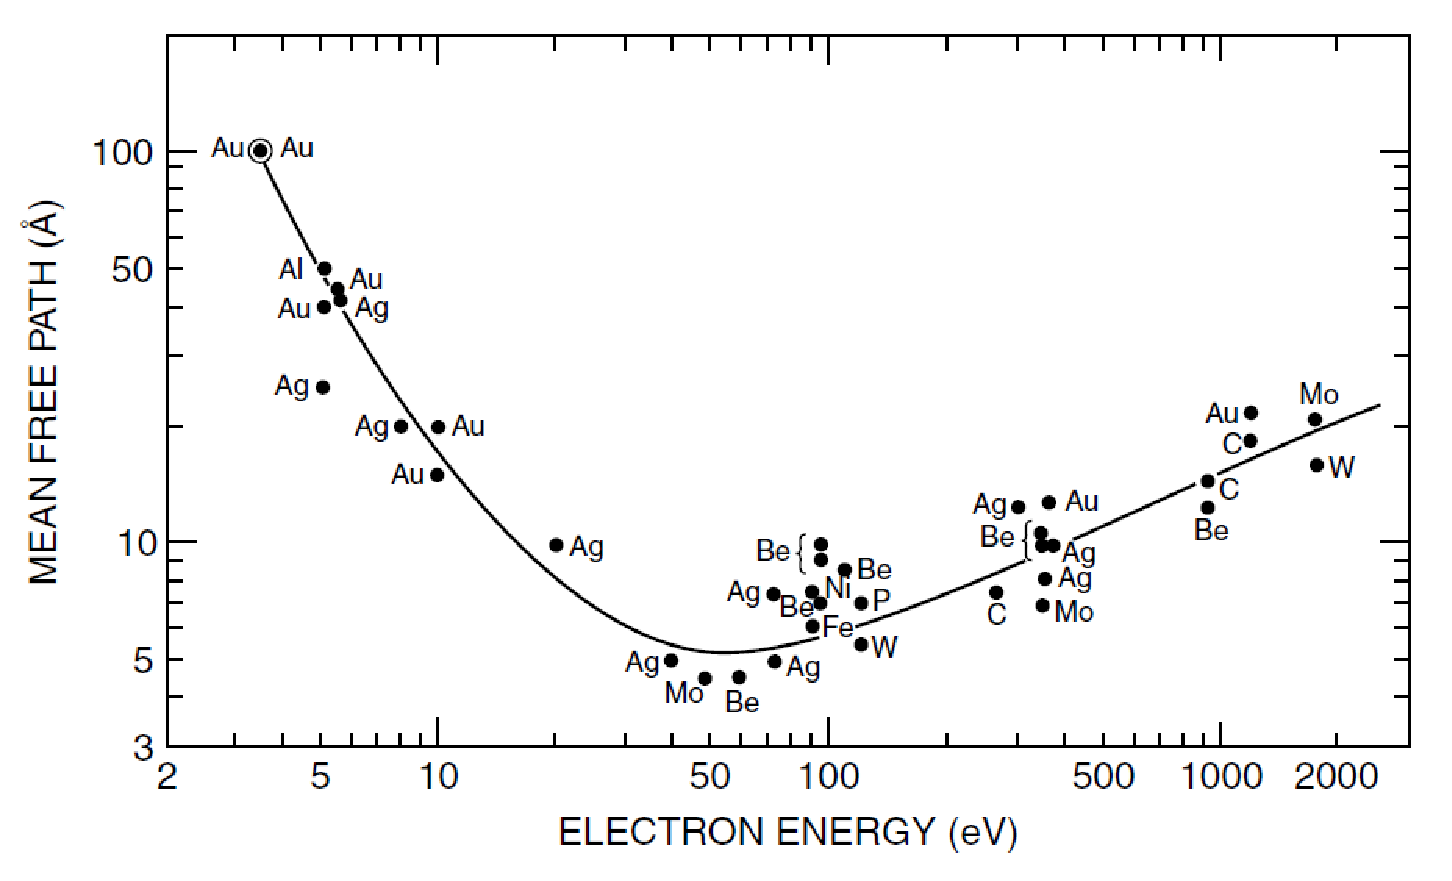
\includegraphics[scale=0.4]{img/ucurve}
\caption{Universal curve of electron escape depth \label{fig:ucurve}}
\end{figure}

\subsection{Inner-Shell Excitations and the Auger Effect}

A particle of high enough energy can scatter with an inner shell electron, exciting it enough that it leaves the atom and becomes free, leaving a hole. The atom is now in an unstable state and will relax by either by emitting an X-ray photon or an Auger electron, both possible relaxation processes are shown in~\ref{fig:aauger}.

In the X-ray relaxation process is relatively simple. An electron from a higher shell takes the place of the core electron and emits a photon in an energy range between $100\,$eV and some MeV, depending on the element. The spectrum of this process is discrete and the remaining atom is singly ionized.

The second possible relaxation process is the emission of an Auger electron. In this relaxation process an electron from a higher shell fills the core hole and the emitted photon is absorbed by another electron in a higher shell that is thus excited in the continuum. The resulting atom is doubly ionized. A schematic for the process is shown in~\ref{fig:aauger} using the example of the $KL_{1}K_L{3}$ process. The electron in the $K$-shell is excited into the continuum, an $L_1$ electron takes its place and another $l_3$ is emitted as a result.

The energy of the emitted Auger electron is given by
\begin{equation}
E_{kin} = E(K)-E(L)-E'(L') = E(K)-E(L)-E(L')-C(LL',T)+R
\end{equation}
where the $E(K)$ is the binding energy of the core electron, $E(L)$ is the binding energy of the electron filling the core hole. $E'(L')$ is the effective binding energy of the electron that is emitted as Auger electron. The effective binding energy consists of the binding energy of the shell $E(L')$, a coupling energy between the holes at $L$ and $L'$ and the final state $T$ and a so-called electronic relaxation $R$. It is important to note that the kinetic energy of the Auger electron is only dependent on the participating states of the Auger process and not on the energy of the particle that initially excites the core electron.

The dominant relaxation process is dependent on the atomic mass number $Z$, whereas for lighter atoms the relaxation by emission of an Auger electron dominates over X-ray emission.

\begin{figure}
\centering
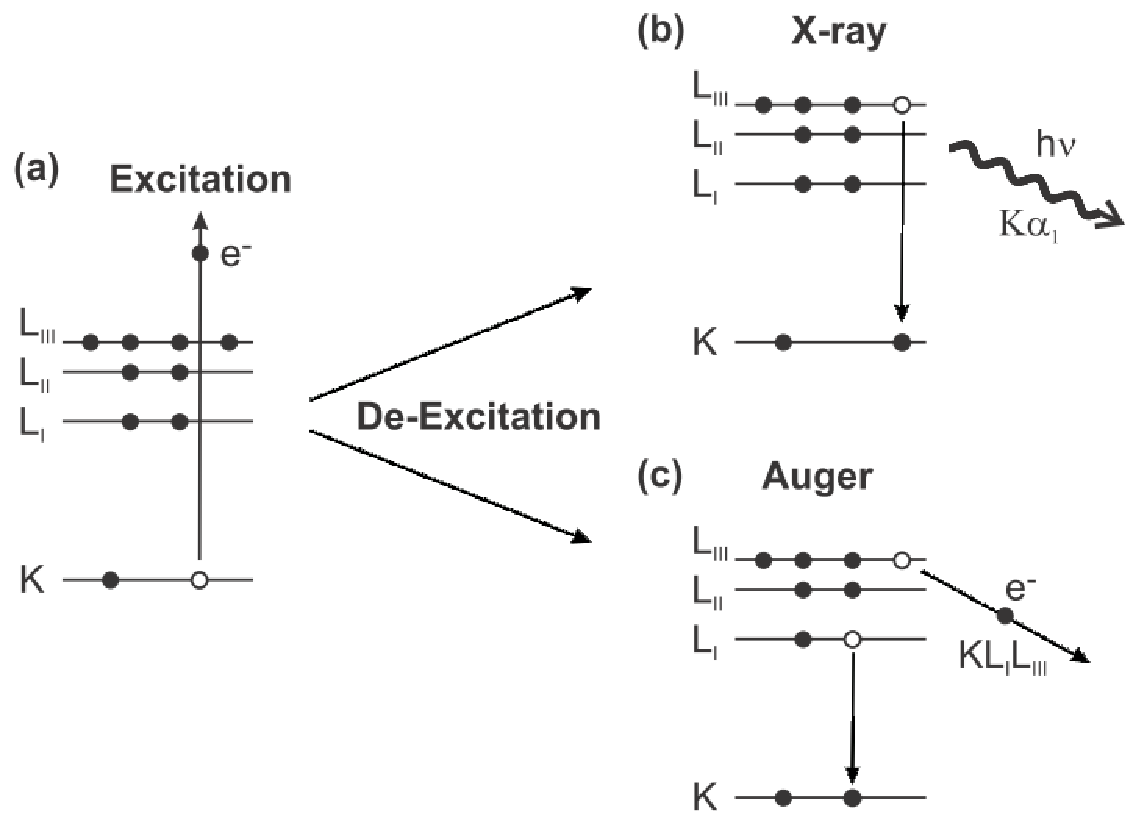
\includegraphics[scale=0.4]{img/auger}
\caption{Auger KLM process and emission of an X-ray \label{fig:aauger}}
\end{figure}


\subsection{Spin-Orbit Coupling}

To fully describe an electron's energy in an atom one has to account for magnetic moments of the electron. Each electron has a magnetic moment due to its orbital movement in the atom and another one due to its spin. All of these magnetic moments of all electrons interact and lead to energy shifts in the spectra. For light atoms the spin-orbit interaction can be approximated by an interaction of the total angular momentum and the total spin (L-S-coupling), which is possible when the coupling of individual spins and orbital angular momenta is negligible. The part of the Hamiltonian describing spin-orbit coupling is then given by
\begin{equation}
H_{SL} = - \frac{\mu_B}{\hbar m_e e c^2}\frac{1}{r}\frac{\partial V(r)}{\partial r} \boldsymbol{L}\cdot\boldsymbol{S},
\end{equation}
where $\mu_B$ is the Bohr magneton, $m_e$ is the electron mass, $e$ is the elementary charge, $c$ is the speed of light, $V$ is the core potential and $r$ is the distance of the electron to the nucleus.

For heavier atoms the coupling between individual spin and orbital momenta is non-negligible and a better approximation is the coupling of individual total angular moment $J_i=L_i+S_i$, this is called J-J-coupling.

Since Aluminum is a light element it is best described with L-S-coupling. The appropriate selection rules are thus $\Delta S=0$ and $\Delta L = 0, \pm 1$.

\subsection{X-Ray Notation}

For historical reasons X-ray notation is used in describing Auger processes. Thus the principal quantum number $n$ is represented by the letters K, L, M$\ldots$ for the numbers $1, 2, 3 \ldots$ and a subscript to those letters to associate a term symbol to those states. The states $S_{1/2}$ are given the subscript 1, $P_{1/2}$ is given the subscript 2, $P_{3/2}$ is given the subscript 3, and so on. Hence the state $L_2$ is equivalent to $2P_{1/2}$ in spectroscopic notation.

\subsection{Plasmons}

A plasmon is a quasi-particle coming up in condensed matter, describing quantized plasma oscillations, i.e. oscillations of the electron gas as a whole. The excitation energy of plasmons is specific to all materials and are given by the materials plasma frequency. For a free electron gas the bulk plasma frequency is given by
\begin{equation}
\omega_{b} = \sqrt{\frac{e^2 n}{m_e \epsilon_0}},
\end{equation}
where $e$ is the elementary charge, $\epsilon_0$ the permittivity of free space, $m_e$ the mass of the electron and $n$ the conduction electron density. 

Plasmon that appear on the interface between two materials and are confined to a surface are called surface plasmons. Because of their lower dimensionality the plasma frequency is lower than for the three-dimensional case, with $\omega_{s} = \omega_{b}/\sqrt{2}$. This excitation can be measured in the EELS part of present experiment as intensity peaks in the energy loss spectra at the energies $E=n \hbar \omega_{s}$ with $n \in \mathbb{N}$.

\section{Experimental Setup}

In this section we will describe shortly the machinery and techniques used in this experiment.

\subsection{Ultra High Vacuum (UHV)}

This experiment needs an ultra high vacuum environment for two reasons. First, electrons have very short mean free path in matter, second, the higher the pressure the faster gas atoms from the rest atmosphere in the chamber adsorb to the sample.

The adsorption is described by the unit Langmuir L, one Langmuir describes the adsorption of a mono-atomic layer on a sample and is obtained at a pressure of $10^{-8}\,$torr after $100\,$s.

The ultra high vacuum is usually obtained by the use of a membrane, a turbo molecular and an ion getter pump. In our case the turbo molecular pump was broken, which is why we experimented at a pressure of $4.3 \cdot 10^{-8}\,$mbar and not the usually recommended $10^{-10}\,$mbar.

\subsection{Cylindrical Mirror Analyzer}

In this experiment a Cylindrical Mirror Analyzer (CMA) is used to measure the energy of the electrons scattered off our sample. A schematic of the CMA is shown in figure~\ref{fig:cma}.

The CMA consists of two concentric cylinders, with the inner cylinder having two two ring-slits. The electrons coming from the sample pass through the first ring slit into the space between both cylinders in which a negative potential $V_{0}$ is applied, deflecting the path of the electrons. To hit the detector the electrons need to pass the second ring-slit. This combination of ring-slits and application of an electric field allows to measure electrons deflected at specific angles from the sample and with very precise energy ranges.

The detector used in the CMA is a channeltron, which is a continuous version of a dynode electron multiplier. The channeltron is basically a thin glass cone coated with a semiconducting material. The signal is amplified by emission of secondary electrons after, which multiplies the number of electrons in the channeltron that finally arrive at the anode.

The current measured at the detector for a certain applied potential is directly proportional to the number of incoming electrons of a certain energy. The signal to noise ratio of the CMA can be improved by applying an oscillating voltage $V_{osc} \sin \omega t$ on top of the static potential $V_{0}$. The measured current can then be expressed as an expansion around the static potential.
\begin{equation}
I = I(V_{0}) + \frac{\mbox{d} I}{\mbox{d} V} V_{osc} \sin \omega t + \ldots
\end{equation}
Knowing the frequency $\omega$ of the applied oscillating potential the signal can be filtered out by the use of a Lock-in amplifier. We can thus extract the amplitude of the oscillating signal, which is, as already mentioned, proportional to the number of electrons of a certain energy:
\begin{equation}
\frac{\mbox{d} I}{\mbox{d} V} \propto \frac{\mbox{d} N}{\mbox{d} E}
\end{equation}

\begin{figure}
\centering
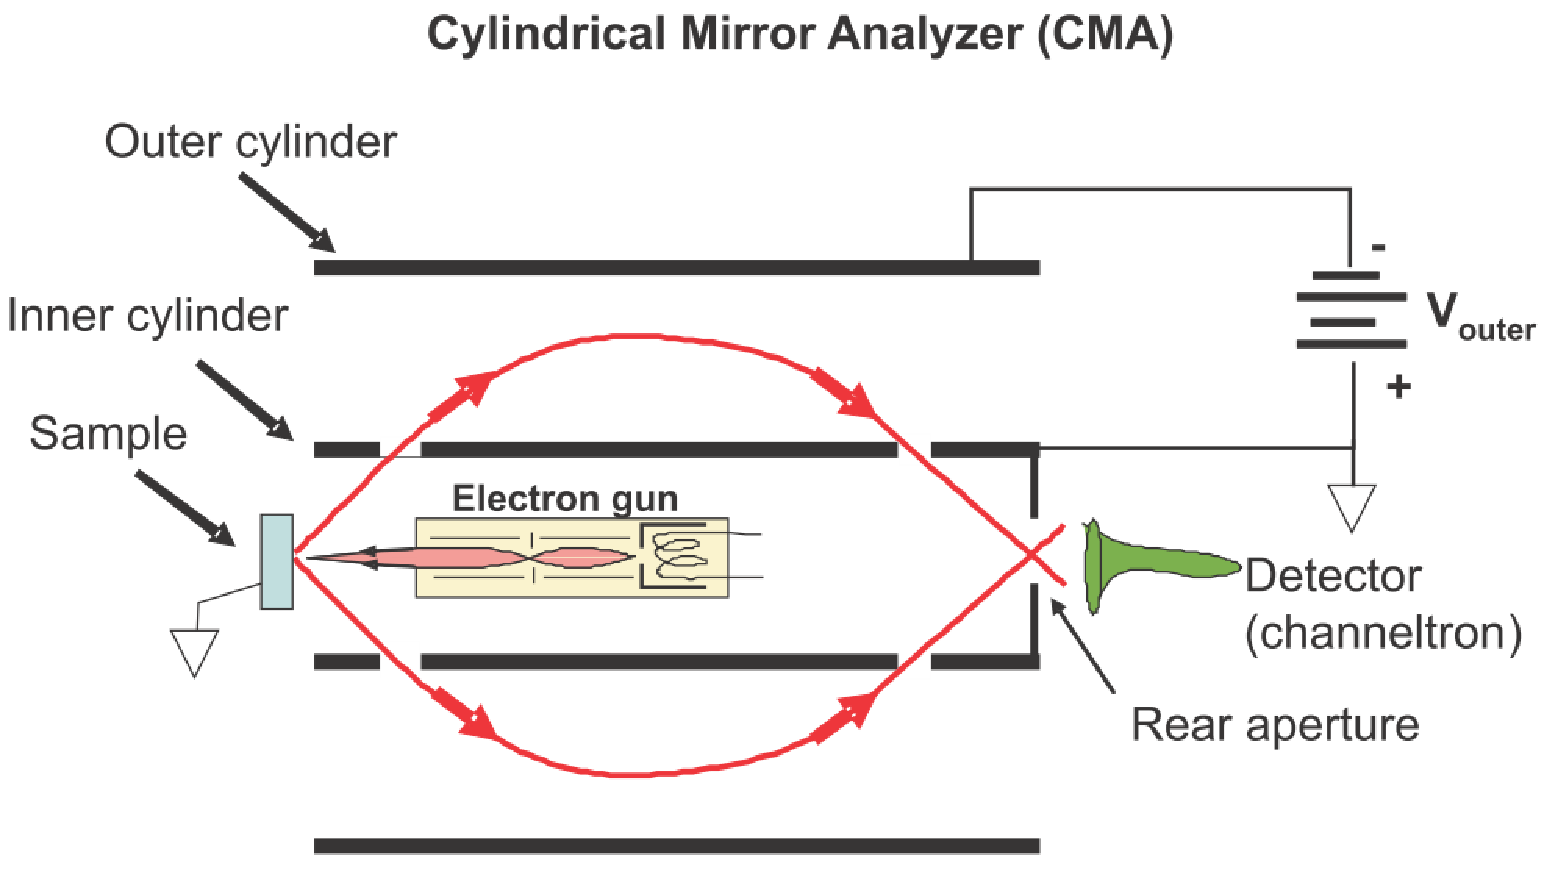
\includegraphics[scale=0.35]{img/cma}
\caption{Cylindrical mirror analyzer \label{fig:cma}}
\end{figure}

\begin{figure}
\centering
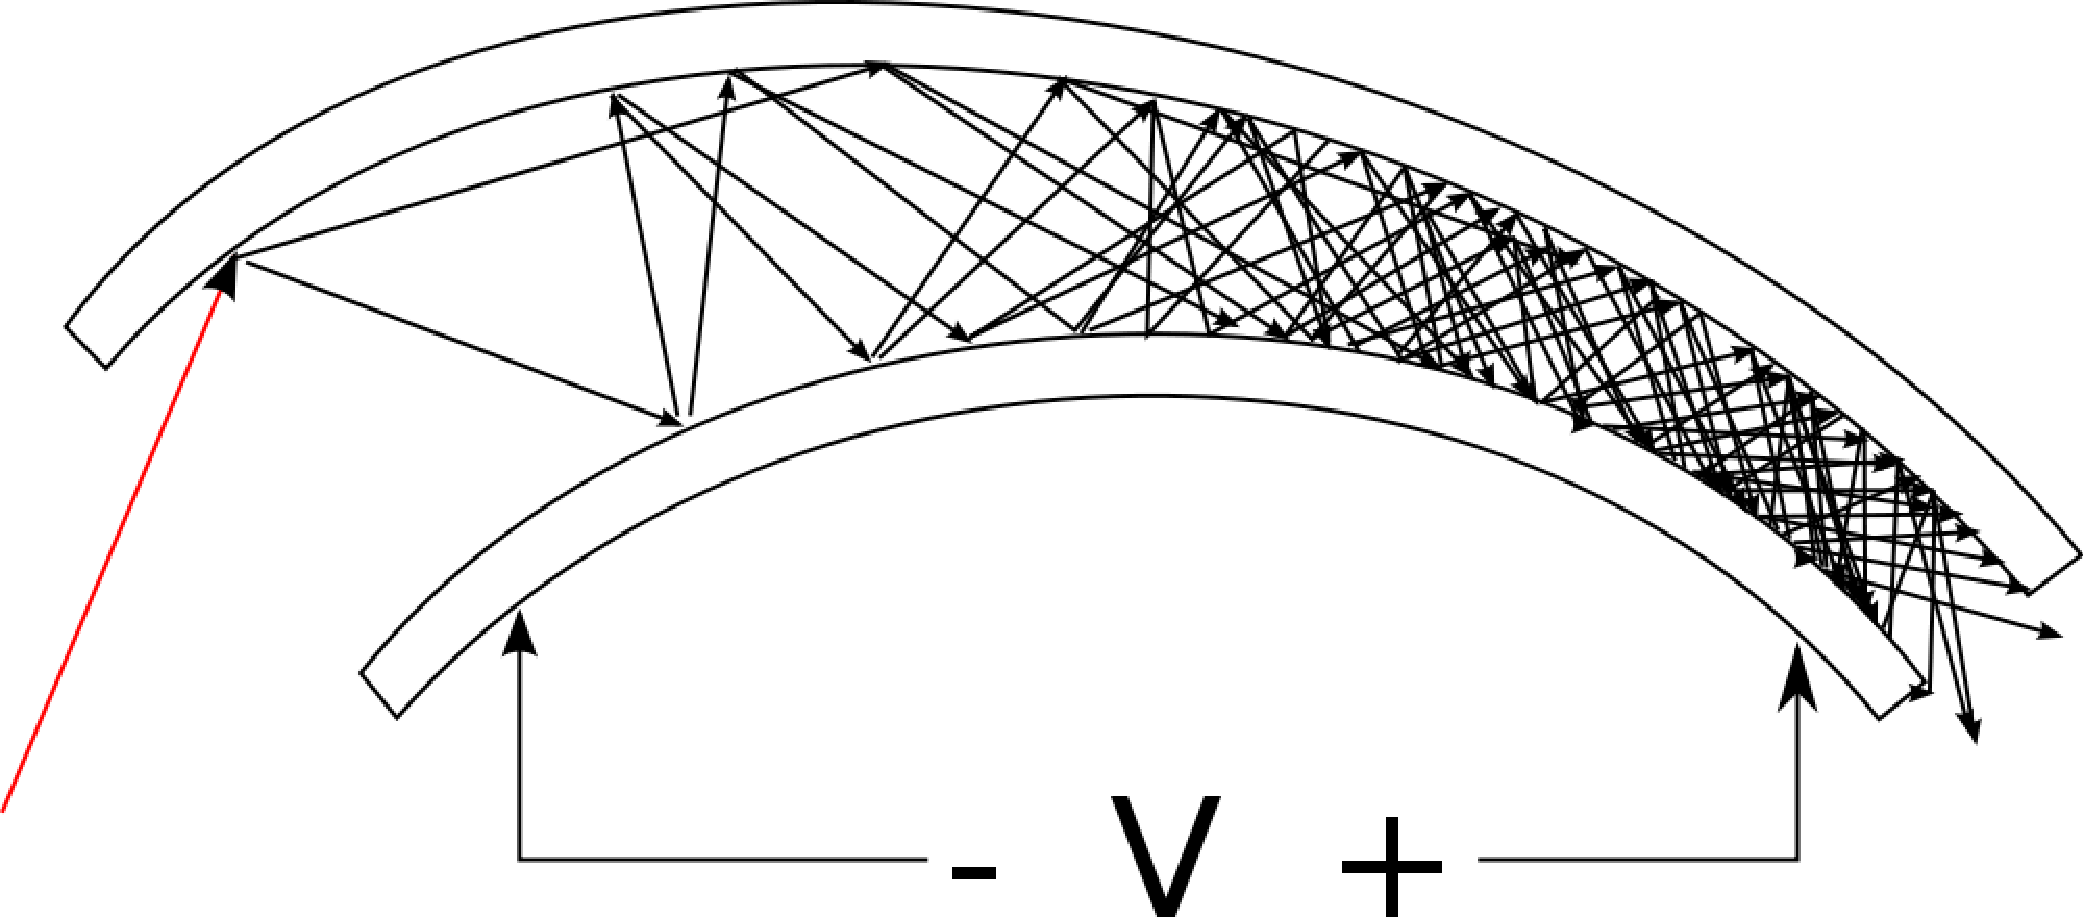
\includegraphics[scale=0.25]{img/channeltron}
\caption{Channeltron \label{fig:ct}}
\end{figure}

\section{Data Analysis}

In this section we will analyze the measured data. We will first look at the cleaning of the sample, will then look at the excitation of bulk and surface plasmons, obtained by Electron Energy Loss spectroscopy, and end this section with an analysis of the Auger spectrum of aluminum.

If not mentioned otherwise we use Gaussian error propagation and least square algorithms for fitting. Also, all spectra were done with an energy step size of $1\,$eV and by averaging over $3$ measurements.

The errors given for all obtained values are obtained from the uncertainty in fit parameters, these uncertainties usually understate the actual errors, but are used for consistency, since they are the only easily quantifiable errors, because errors and noise in our measurements are nearly eliminated by the averaging process.

\subsection{Sample Cleaning}

\begin{figure}
\centering
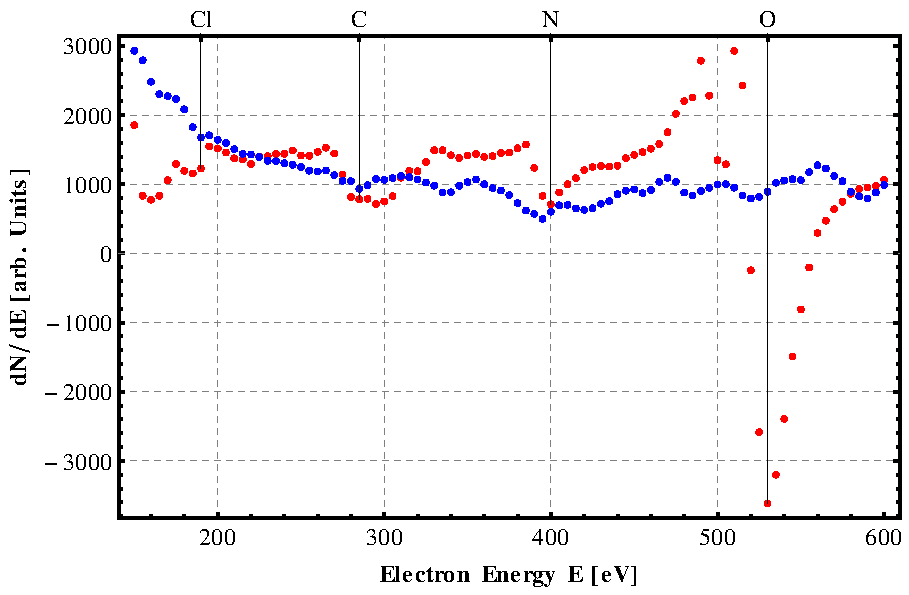
\includegraphics[scale=0.6]{img/cleaning}
\caption{Exemplary differential Auger spectra before (red) and after (blue) cleaning. \label{fig:cleaning}}
\end{figure}

Figure~\ref{fig:cleaning} shows the part of the Auger spectrum of the aluminum sample, where peaks resulting from impurities can be found. Using~\cite{handbook} we can identify oxygen, nitrogen, carbon and possibly chlorine as impurities. Nitrogen and oxygen as main parts of air are not surprising but carbon and chlorine are, since they are not part of air.

Having filed on the sample for over half an hour and seeing  peaks almost vanish and then reappear shortly thereafter, we think that these peaks result from filing some parts of the sample holder, since it is quite easy to miss the sample with the file.

Furthermore we have to conclude, that the cleaning of the sample is rather useless, since the pressure in the chamber ($p = 4.3 \cdot 10^{-8}$) is too high for the proper conductance of the experiment, since after two minutes, this leads to the adsorption of nearly four monolayers of oxygen:
\begin{equation}
4.3 \cdot 10^{-8}\,\mbox{mbar} \times 120\,\mbox{s} = 3.87\,\mbox{L},
\end{equation} 
which we could verify in so far, as the state of the oxygen peak at the end of the cleaning process (blue in figure~\ref{fig:cleaning}) had changed back to state before the cleaning (red in figure~\ref{fig:cleaning}).

Nevertheless the experiment could be conducted and lead to qualitatively good results, as will be shown in the following section, but we see the described problems as a major error source.

\subsection{Plasmons}

The Electron Energy Loss Spectroscopy experiments were done after taking the Auger spectrum of the sample. 

We think, that the excitation of bulk plasmons is needed to understand the results of the Auger spectrum, which is why we will discuss the plasmon excitations first.

The electron gun energy was adjusted to $1\,$kV for the spectroscopy of the bulk plasmons and to $0.2\,$kV for the surface plasmon spectroscopy. Both energies are too low to excite Auger electrons, so that the Auger effect can be excluded for the measured phenomena and they have to be explained by plasmon excitation.

\subsubsection{Bulk Plasmons}

Figure~\ref{fig:bulkpeaks} shows the differential and the integrated spectrum of the EELS of bulk plasmon excitation. 

To obtain the bulk plasmon excitation energy we fitted the first four peaks from the right with gaussians, since they were the only peaks, that exhibited a definite shape, i.e. had a discernible midpoint. The peak positions can be found in table~\ref{tab:bulkpeaks}.

Using the Gaussian midpoint positions, we then obtained the following value for the excitation energy by linear regression:
\begin{equation}
\Delta E_{bulk} = (14.19 \pm 0.05)\,\mbox{eV}.
\end{equation}

This value does not agree with the literature value of $15.3\,$eV~\cite{plasmonpaper}, but is at least qualitatively in the vicinity of the literature value. It is possible that this is due to the contamination of the surface with oxygen, although this seems unlikely for the excitation of bulk plasmons. Another possible source of error can be in our energy detector. This will be discussed later in the section on the Auger spectrum.

\begin{figure}
\centering
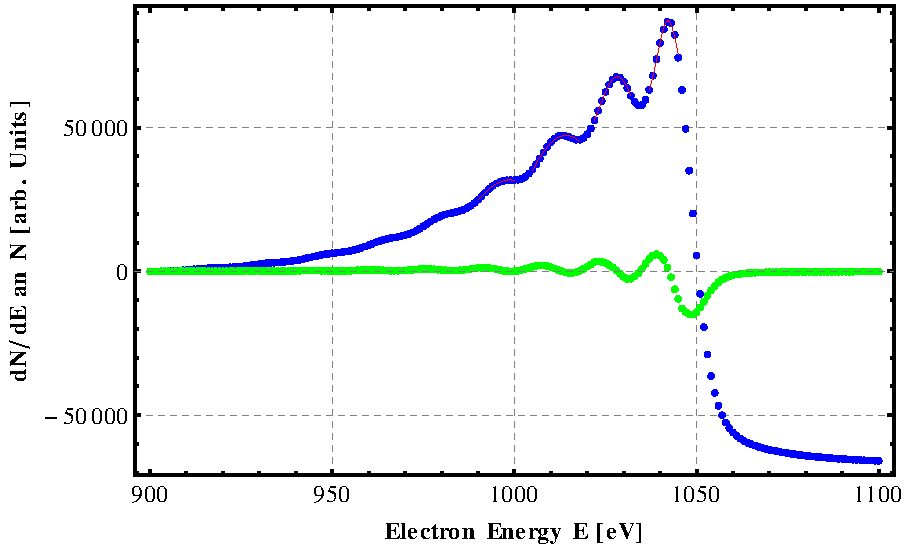
\includegraphics[scale=0.6]{img/bulkpeaks}
\caption{Integrated (blue) and differential (green) electron energy loss spectrum for the bulk plasmon measurement. Fits for peak positions are plotted on top of the integrated spectrum in red. \label{fig:bulkpeaks}}
\end{figure}


\begin{table}
\begin{center}
\begin{tabular}{lcc}
\toprule
Peak Position E [eV]\\
\midrule
\phantom{0}998.66 $\pm$ 0.17 \\
1014.17 $\pm$ 0.19 \\
1028.27 $\pm$ 0.02 \\
1042.15 $\pm$ 0.06 \\
\bottomrule
\end{tabular}
\end{center}
\par
\caption{Peak positions of bulk plasmons. \label{tab:bulkpeaks}}
\end{table}


\subsection{Surface Plasmons}

The differential and integrated spectrum for the surface plasmon EELS can be found in figure~\ref{fig:surfacepeaks}.

We can see, that the integrated spectrum does not exhibit many features, which is why we were only able to successfully fit two peaks: The well-pronounced major peak on the right, which is due to, more or less, elastically back-scattered electrons, and the misshapen peak to its right.
Further analysis showed, that this peak is a superposition of two peaks, one describing the excitation of the surface plasmon and one describing the excitation of a bulk plasmon.

All three peaks were fitted with gaussians, the respective peak positions can be found in table~\ref{tab:surfacepeaks}. The resulting excitation energies are:
\begin{IEEEeqnarray}{rCl}
\Delta E_{bulk} & = & (14.3 \pm 0.5)\,\mbox{eV}, \\
\Delta E_{surf} & = & (\phantom{0}9.6 \pm 0.3)\,\mbox{eV}.
\end{IEEEeqnarray}
Both numbers are not consistent with the excitation energies of $15.3\,$eV and $10.8\,$eV for bulk an surface plasmons from~\cite{plasmonpaper}, but the bulk plasmon excitation energy is consistent with the one obtained earlier and both are in the vicinity of the literature value. 

The same possible sources as for the bulk plasmon EELS apply, but surface contamination is naturally a more probable error source in this case.

\begin{figure}
\centering
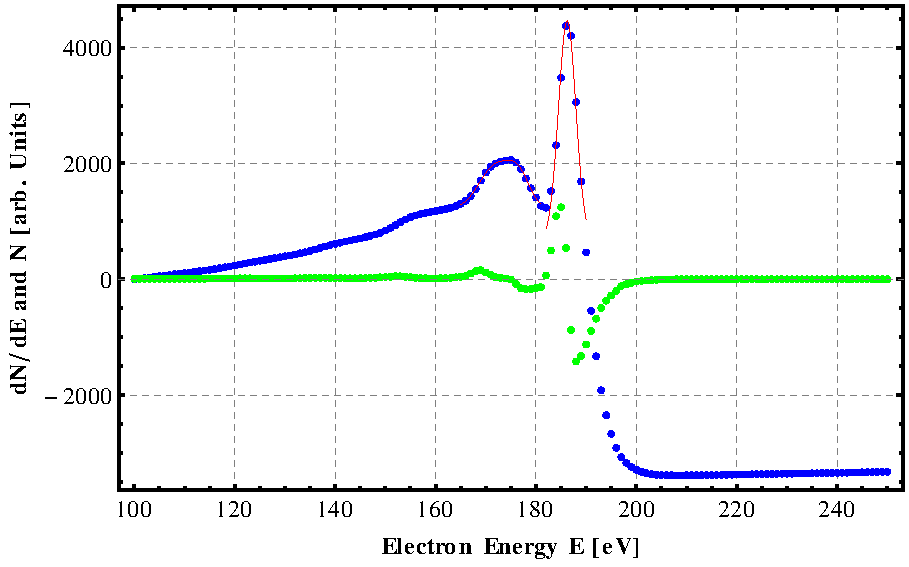
\includegraphics[scale=0.6]{img/surfacepeaks}
\caption{Integrated (blue) and differential (green) electron energy loss spectrum for the surface plasmon measurement. Fits for peak positions are plotted on top of the integrated spectrum in red. \label{fig:surfacepeaks}}
\end{figure}

\begin{table}
\begin{center}
\begin{tabular}{lcc}
\toprule
Peak Position E [eV]\\
\midrule
171.95 $\pm$ 0.40 \\
176.67 $\pm$ 0.25 \\
186.23 $\pm$ 0.12 \\
\bottomrule
\end{tabular}
\end{center}
\par
\caption{Peak positions of surface plasmons. \label{tab:surfacepeaks}}
\end{table}

\subsection{Auger Spectrum}

The Auger spectrum of the sample was taken with an electron gun energy of $4.8\,$eV. The interesting part of the differential spectrum can be found in figure~\ref{fig:augerpeaks}. 

We fitted all minima and maxima of the differential spectrum with gaussians to obtain their position in the spectrum. The appropriate fit parameters can be found in table~\ref{tab:augerpeaks}.

The distribution of the minima, agrees qualitatively very well, with the literature values form~\cite{handbook}, but they seem to be shifted by a constant additive factor to higher energies. If we artificially put the last minimum on its literature value and use this offset to recalibrate the spectrum, all minima agree remarkably well, with their literature values.

The reason for this shift could have several reasons. Firstly it could be because of the contamination of the surface with oxygen. Another reason could be systematic error in the analyzer, for example due to insufficient positioning of the sample.

Figure~\ref{fig:intaugerpeaks} shows the integrated Auger spectrum of our sample, which should be used to obtain the peaks for the KLL transitions in aluminum. Unfortunately this spectrum is unusable, since only the two rightmost peaks are pronounced enough to be discernible.To solve this problem we took the maxima and minima positions in figure~\ref{fig:augerpeaks} and took the average between a minimum and its preceding maximum, which gives a rough estimate for the position of a peak in figure~\ref{fig:intaugerpeaks}. The estimated peak positions can be found in the lower section of table~\ref{tab:augerpeaks}. 

The estimated peak positions in the integrated Auger spectrum need to be identified with a Auger KLL transition from table~\ref{tab:augerpeakscomp}. Possible identifications, taking possible energy losses due to plasmon excitation into account, can be found in table~\ref{tab:identification}, although for some measure peaks several transitions come into consideration, but cannot be discerned. This may be due to two neighboring peaks being combined to one peak of average energy.

\begin{figure}
\centering
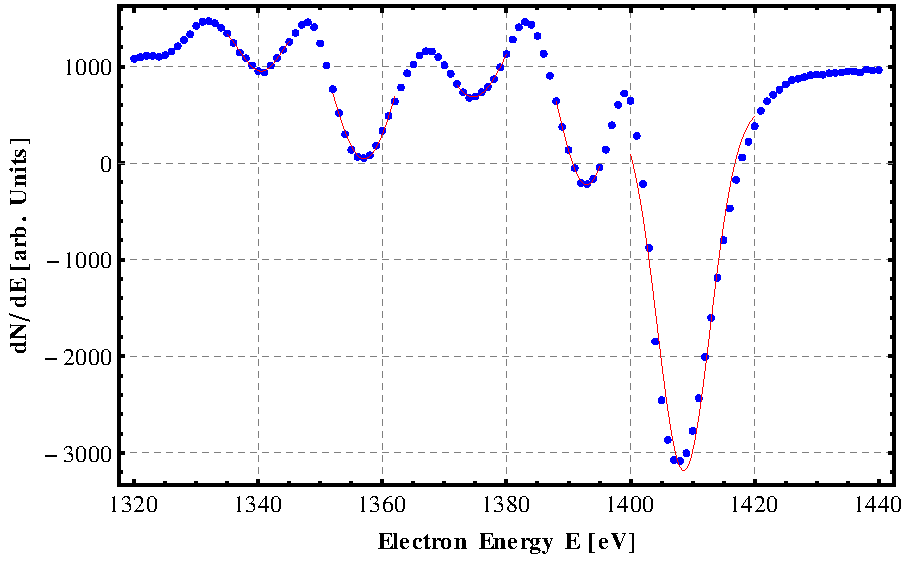
\includegraphics[scale=0.6]{img/augerpeaks}
\caption{Differential Auger spectrum for aluminum. Fits for the maxima and minima are plotted on top of the spectrum in red. \label{fig:augerpeaks}}
\end{figure}

\begin{figure}
\centering
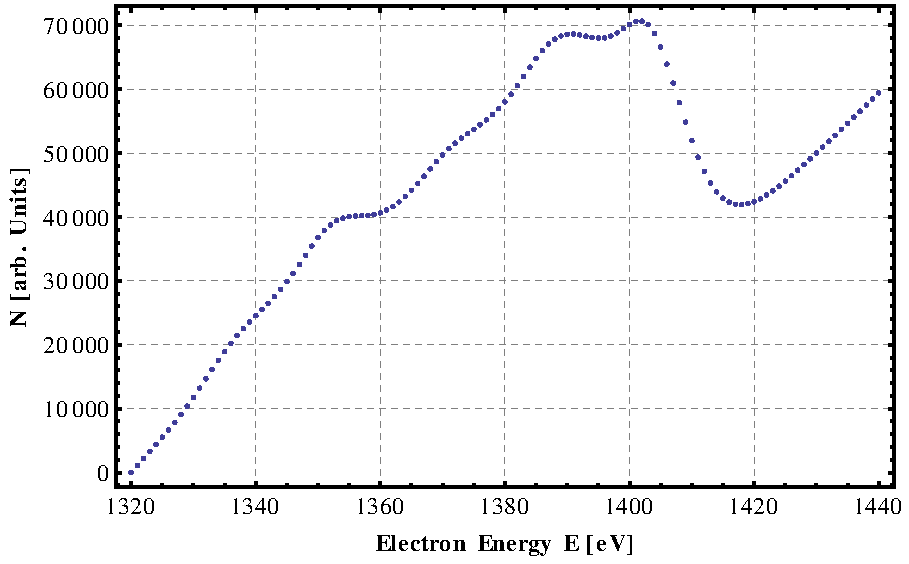
\includegraphics[scale=0.6]{img/intaugerpeaks}
\caption{Integrated Auger spectrum for aluminum. \label{fig:intaugerpeaks}}
\end{figure}


\begin{table}
\begin{center}
\begin{tabular}{lcc}
\toprule
peak position  [eV]                    & recalibrated peak position [eV]        & literature value [eV]\\
\midrule
1340.45 $\pm$ 0.07                     & 1327.86 $\pm$ 0.07                     & 1329 \\
1357.08 $\pm$ 0.07                     & 1344.49 $\pm$ 0.07                     & 1345 \\
1374.66 $\pm$ 0.08                     & 1362.07 $\pm$ 0.08                     & 1364 \\
1392.93 $\pm$ 0.04                     & 1380.34 $\pm$ 0.04                     & 1380 \\
1408.6\phantom{0} $\pm$ 0.2\phantom{0} & 1396.0\phantom{0} $\pm$ 0.2\phantom{0} & 1396 \\
\midrule
1331.8\phantom{0} $\pm$ 0.1\phantom{0} & 1319.2\phantom{0} $\pm$ 0.1\phantom{0} & \\
1347.0\phantom{0} $\pm$ 0.2\phantom{0} & 1334.5\phantom{0} $\pm$ 0.2\phantom{0} & \\
1367.54 $\pm$ 0.05                     & 1354.95 $\pm$ 0.0                      & \\
1383.05 $\pm$ 0.03                     & 1370.46 $\pm$ 0.0                      & \\
1398.5\phantom{0} $\pm$ 0.2\phantom{0} & 1385.89 $\pm$ 0.2                      & \\
\midrule
1336.1\phantom{0} $\pm$ 0.2\phantom{0} & 1323.5\phantom{0} $\pm$ 0.2\phantom{0} & \\
1352.1\phantom{0} $\pm$ 0.2\phantom{0} & 1339.5\phantom{0} $\pm$ 0.2\phantom{0} & \\
1371.1\phantom{0} $\pm$ 0.2\phantom{0} & 1358.5\phantom{0} $\pm$ 0.2\phantom{0} & \\
1388.0\phantom{0} $\pm$ 0.2\phantom{0} & 1375.4\phantom{0} $\pm$ 0.2\phantom{0} & \\
1403.5\phantom{0} $\pm$ 0.2\phantom{0} & 1390.9\phantom{0} $\pm$ 0.2\phantom{0} & \\
\bottomrule
\end{tabular}
\end{center}
\par
\caption{Upper part: minimum positions of aluminum auger spectrum. Recalibrated peak positions shifted that last peak coincides with literature value. Literature values taken from~\cite{handbook}. Middle part: maximum positions of aluminum auger spectrum. Lower part: means of minimum and preceding maximum as approximation for peak position in integrated spectrum.\label{tab:augerpeaks}}
\end{table}



\begin{table}
\begin{center}
\begin{tabular}{lccc}
\toprule
Auger Line                & Energy E [eV] & $+B_{1}$ & $+B_{2}$ \\
\midrule
$KL_{1}L_{2,3} (^{1}P)$   & 1342.3        & 1328.1   & 1313.9 \\
$KL_{1}L_{2,3} (^{3}P)$   & 1358.5        & 1344.3   & 1330.1 \\
$KL_{2,3}L_{2,3} (^{1}S)$ & 1386.6        & 1372.4   & 1358.2 \\
$KL_{2,3}L_{2,3} (^{1}D)$ & 1393.5        & 1379.2   & 1365.0 \\
$KL_{2,3}L_{2,3} (^{3}P)$ & 1398.1        & 1383.9   & 1369.7 \\
\bottomrule
\end{tabular}
\end{center}
\par
\caption{Auger peak energies from~\cite{augerpaper} with corrections for subsequent excitation of up to two bulk plasmons. \label{tab:augerpeakscomp}}
\end{table}

\begin{table}
\begin{center}
\begin{tabular}{lcc}
\toprule
Auger Line                                  & Theoretical Energy [eV] & Measured Energy [eV] \\
\midrule
$KL_{1}L_{2,3}: ~~\phantom{P}^{1}P + B_{1}$ & 1328.1                  & 1323.5 $\pm$ 0.2 \\
$KL_{1}L_{2,3}: ~~\phantom{P}^{1}P$         & 1342.3                  & 1339.5 $\pm$ 0.2 \\       
$KL_{1}L_{2,3}: ~~\phantom{P}^{3}P$         & 1358.5                  & 1358.5 $\pm$ 0.2 \\
$KL_{2,3}L_{2,3}: \phantom{P}^{1}S + B_{2}$ & 1358.2                  & 1358.5 $\pm$ 0.2 \\
$KL_{2,3}L_{2,3}: \phantom{P}^{1}S + B_{1}$ & 1372.4                  & 1375.4 $\pm$ 0.2 \\        
$KL_{2,3}L_{2,3}: \phantom{P}^{1}D + B_{1}$ & 1379.4                  & 1375.4 $\pm$ 0.2 \\
$KL_{2,3}L_{2,3}: \phantom{P}^{1}S$         & 1386.6                  & 1390.9 $\pm$ 0.2 \\        
$KL_{2,3}L_{2,3}: \phantom{P}^{1}D$         & 1393.5                  & 1390.9 $\pm$ 0.2 \\        
\bottomrule
\end{tabular}
\end{center}
\par
\caption{Auger peak energies from~\cite{augerpaper} with corrections for subsequent excitation of up to two bulk plasmons. \label{tab:identification}}
\end{table}


\section{Conclusion}

We performed Auger and Electron Energy Loss Spectroscopy on an aluminum sample and observed the Auger spectrum of aluminum as well as the excitation of bulk and surface plasmons. 

Whereas the obtained differential Auger spectrum, with an offset in energy that had to be recalibrated, seemed in good qualitative agreement with the literature, the integrated Auger spectrum was unusable for evaluation. An approximative usage of the differential Auger spectrum allowed us to identify Auger KLL transitions, that agreed with literature values~\cite{augerpaper}.

The plasmon excitation energies ($\Delta E_{bulk} = (14.19 \pm 0.05)\,\mbox{eV}$ and $\Delta E_{bulk} = (9.6 \pm 0.3)\,\mbox{eV}$) obtained from the EEL spectra were not in agreement with literature values~\cite{plasmonpaper}. One reason for the large deviation in the value of the surface plasmon excitation energy might be due to contamination of the surface with oxygen but also to the fact, that we were only able to measure one surface plasmon.

The experimental setup would allow for much better values, since the accuracy of the measurement devices is quite good. It is very problematic, though, that the vacuum chamber lacks the turbomolecular pump, which is the reason for the high pressure in the chamber. Another improvement could be made in the angular positioning of the sample, since this might have an effect on the measurements of the CMA. A further improvement to the experiment could be made by exchanging the file for a sputter gun.

\nocite{skript}
\nocite{augerpaper}
\nocite{plasmonpaper}
\nocite{handbook}
\nocite{ben}
\nocite{christian}

\bibliographystyle{plainnat}
\bibliography{auger}

\end{document}
